%% ----------------------------------------------------------------
%% Thesis.tex -- MAIN FILE 
%% ---------------------------------------------------------------- 

% Set up the document
\documentclass[a4paper, 11pt, oneside]{Thesis}  % Use the "Thesis" style, based on the ECS Thesis style by Steve Gunn
\graphicspath{Figures/}  % Location of the graphics files (set up for graphics to be in PDF format)
% Table configuration packages
\usepackage{array,graphicx}
\usepackage{booktabs}
\usepackage{pifont}
\usepackage{libertine}
\usepackage{tabu}
\usepackage{longtable}
\usepackage[table]{xcolor}
\usepackage{tcolorbox}
\usepackage{textcomp}
\usepackage{multicol}
% My additions
\usepackage{amsmath}
\usepackage[utf8]{inputenc}
\usepackage{pgfplots}
\DeclareUnicodeCharacter{2212}{−}
\usepgfplotslibrary{groupplots,dateplot}
\usetikzlibrary{patterns,shapes.arrows}
\pgfplotsset{compat=newest}
% \usepackage[table,xcdraw]{xcolor}
% \newtheorem{definition}{Definition}
%

\makeatother

% Include any extra LaTeX packages required
\usepackage[square, numbers, comma, sort&compress]{natbib}  % Use the "Natbib" style for the references in the Bibliography
\usepackage{verbatim}  % Needed for the "comment" environment to make LaTeX comments
\usepackage{float} % To keep figures in place
\hypersetup{urlcolor=black, colorlinks=false, pdfborder = {0 0 0}}  % Colours hyperlinks in blue
% Define enumerated description lists
\usepackage{enumitem}
\newcounter{descriptcount}
\newcounter{descriptcount2}
\newlist{enumdescript}{description}{2}
\setlist[enumdescript,1]{%
  before={\setcounter{descriptcount}{0}%
          \renewcommand*\thedescriptcount{\arabic{descriptcount}.}}
  ,font=\bfseries\stepcounter{descriptcount}\thedescriptcount~
}
\setlist[enumdescript,2]{%
  before={\setcounter{descriptcount2}{0}%
          \renewcommand*\thedescriptcount{\roman{descriptcount2}.}}
  ,font=\bfseries\stepcounter{descriptcount2}\thedescriptcount~
}
 

 
%% ----------------------------------------------------------------
\begin{document}

% For changes in supervisor, degree type, research group, etc. please change the Thesis.cls file
\frontmatter      % Begin the book's numbering; frontpage
%
%\pagenumbering{arabic}

% Set up the Title Page
\title  {Thesis Title}

\authors  {\texorpdfstring
            {\href{mailto:itsouros@auth.gr}{Iakovos Marios Tsouros}}
            {Author's Name}
            }
\addresses  {\groupname\\\deptname\\\univname}  % Do not change this here, instead these must be set in the "Thesis.cls" file, please look through it instead
\date       {Date}
\subject    {}
\keywords   {}

\maketitle

%% ----------------------------------------------------------------

\setstretch{1.3}  % It is better to have smaller font and larger line spacing than the other way round

% Define the page headers using the FancyHdr package and set up for one-sided printing
\fancyhead{}  % Clears all page headers and footers
\rhead{\thepage}  % Sets the right side header to show the page number
\lhead{}  % Clears the left side page header

\pagestyle{fancy}  % Finally, use the "fancy" page style to implement the FancyHdr headers

%% ----------------------------------------------------------------
% Declaration Page required for the Thesis, your institution may give you a different text to place here
\Declaration{

\addtocontents{toc}{\vspace{1em}}  % Add a gap in the Contents, for aesthetics

I, [author's name], declare that this thesis titled, [thesis title] and the work presented in it are my own. I confirm that:

\begin{itemize} 
\item[\tiny{$\blacksquare$}] This work was done wholly or mainly while in candidature for a research degree at this University.
 
\item[\tiny{$\blacksquare$}] Where any part of this thesis has previously been submitted for a degree or any other qualification at this University or any other institution, this has been clearly stated.
 
\item[\tiny{$\blacksquare$}] Where I have consulted the published work of others, this is always clearly attributed.
 
\item[\tiny{$\blacksquare$}] Where I have quoted from the work of others, the source is always given. With the exception of such quotations, this thesis is entirely my own work.
 
\item[\tiny{$\blacksquare$}] I have acknowledged all main sources of help.
 
\item[\tiny{$\blacksquare$}] Where the thesis is based on work done by myself jointly with others, I have made clear exactly what was done by others and what I have contributed myself.
\\
\end{itemize}
 
 
Signed:\\
\rule[1em]{25em}{0.5pt}  % This prints a line for the signature
 
Date:\\
\rule[1em]{25em}{0.5pt}  % This prints a line to write the date
}
\clearpage  % Declaration ended, now start a new page

%% ----------------------------------------------------------------
% The "Funny Quote Page"
\pagestyle{empty}  % No headers or footers for the following pages

\null\vfill
% Now comes the "Funny Quote", written in italics
\textit{Inspiring quote goes here (optional)}

\begin{flushright}
Quote's attribution
\end{flushright}

\vfill\vfill\vfill\vfill\vfill\vfill\null
\clearpage  % Funny Quote page ended, start a new page
%% ----------------------------------------------------------------

% The Abstract Page
\addtotoc{Abstract}  % Add the "Abstract" page entry to the Contents
\abstract{
\addtocontents{toc}{\vspace{1em}}  % Add a gap in the Contents, for aesthetics

Abstract goes here.

}

\clearpage  % Abstract ended, start a new page
%% ----------------------------------------------------------------

\setstretch{1.3}  % Reset the line-spacing to 1.3 for body text (if it has changed)

% The Acknowledgements page, for thanking everyone
\acknowledgements{
\addtocontents{toc}{\vspace{1em}}  % Add a gap in the Contents, for aesthetics
Acknowledgements go here.

}
\clearpage  % End of the Acknowledgements
%% ----------------------------------------------------------------

\pagestyle{fancy}  %The page style headers have been "empty" all this time, now use the "fancy" headers as defined before to bring them back


%% ----------------------------------------------------------------
\lhead{\emph{Contents}}  % Set the left side page header to "Contents"
\tableofcontents  % Write out the Table of Contents

%% ----------------------------------------------------------------
\lhead{\emph{List of Figures}}  % Set the left side page header to "List if Figures"
\listoffigures  % Write out the List of Figures

%% ----------------------------------------------------------------
\lhead{\emph{List of Tables}}  % Set the left side page header to "List of Tables"
\listoftables  % Write out the List of Tables

%% ----------------------------------------------------------------
\setstretch{1.5}  % Set the line spacing to 1.5, this makes the following tables easier to read
\clearpage  % Start a new page
\lhead{\emph{Abbreviations}}  % Set the left side page header to "Abbreviations"
\listofsymbols{ll}  % Include a list of Abbreviations (a table of two columns)
{
\textbf{Acronym} & \textbf{W}hat (it) \textbf{S}tands \textbf{F}or \\
% Abbreviations go here
}

\lhead{}
%% ----------------------------------------------------------------
% End of the pre-able, contents and lists of things
% Begin the Dedication page

\setstretch{1.3}  % Return the line spacing back to 1.3

\pagestyle{empty}  % Page style needs to be empty for this page
\dedicatory{Dedication (optional)}

\addtocontents{toc}{\vspace{2em}}  % Add a gap in the Contents, for aesthetics


%% ----------------------------------------------------------------
\mainmatter	  % Begin normal, numeric (1,2,3...) page numbering
\pagestyle{fancy}  % Return the page headers back to the "fancy" style

% Include the chapters of the thesis, as separate files
% Just uncomment the lines as you write the chapters

\chapter{Introduction} \label{introduction}
\graphicspath{Figures/chapter1/}
\section{Graphs}
In this subsection, the main aspects of graph theory are briefly presented.
\subsection{Introduction}


% \subsubsection{Begginings and historical remarks}


% \subsubsection{Introduction}

In the real world, many problems can be described by a diagram connecting a set of points with
lines, joining pairs of these points, or even creating loops on a single point. A simple example
of that would be a set of points representing people with lines connecting acquintances, or
points representing atoms and lines representing chemical bonds, creating a representation of
a molecule as a graph attribute. In the examples above, the only information contained is whether
two points are associated, with the manner being disregarded. The concept of a graph consists of
a mathematical abstraction of the above. \cite{book:2008}


\begin{definition} \label{u_simple_graph} Mathematically, in its simplest form, a
  \textbf{graph} is an ordered pair\footnotemark{} $G=(V, E)$ of:
  \begin{itemize}
  \item \textbf{V}, a set of vertices (also known as nodes).
  \item $E \subseteq \{\{x, y\} | x,y \in V ~x \neq y \}$, which is the set of \textbf{edges}
    which consists of unordered pairs of vertices that connect two nodes.
  \end{itemize}
\footnotetext{An ordered pair $(a, b)$ is a pair of objects in which the order of
appearance or insertion is significant; the ordered pair $(a, b)$ is different than $(b,
a)$ unless $a=b$. An unordered pair is a set of the form ${a, b}$ is a set having two
elements with no relation between them and ${a, b} = {b, a}$.  }
\end{definition}

This type of object is called an \textbf{undirected simple graph} to avoid confusion
with other types.

\begin{definition}\label{graph_def}
  A \textit{graph} G is an ordered pair $(V(G), E(G))$ consisting of a set
$V(G)$ of \textit{vertices} (also called \textit{nodes} or \textit{points}) and a set
$E(G)$, disjoint from $V(G)$ which consists of \textit{edges} (also called \textit{links}
or \textit{lines}) together with an incidence function $\psi_G$ that associates with each
edge of G an unordered pair of not necesserily distinct vertices of G.  If $e$ is an edge
and $u$ and $v$ are vertices such that $\psi_G ={u, v}$ then $e$ is said to \textit{join}
$u$ and $v$, and the vertices $u$ and $v$ are called the \textit{ends} of $e$. We denote
the numbers of vertices and edges $G$ by $u(G)$ and $e(G)$ which two parameters are called
the \textit{order} and \textit{size} of G, respectively \cite{book:2008}.

  In short, we can define a \textbf{graph} as an ordered triple $G=(V, E, \phi_G)$
consisting of:
  \begin{itemize}
  \item $V$, a set of \textit{vertices}
  \item $E$, a set of \textit{edges}
  \item $\phi_G: E \rightarrow \{\{x, y\} | x, y \in V \; and \; x \neq y\}$ an
\textit{incidence function} mapping every edge to an unordered pair of vertices - an edge
associated with two distinct vertices. The incidence function is a function of the edges.
  \end{itemize} This type of object is called an \textit{undirected multigraph}, to avoid
confusion. Note, that the above definition of the \textit{incidence function} does not
allow for \textit{loops} (mappings of an edge on the same vertex).

A \textit{loop} is a an edge that allows a connection of a vertex to itself and a graph can
be defined to either allow or disallow the presence of loops. Some authors allow for loops
to exist on \textit{multigraphs} \cite{article:bollobas}, while other consider these kind
of graphs to exist in a different category, called \textit{pseudographs} \cite{book:Gary}.
Allowing loops requires modifying the incidence function so they can be supported. The new
incidence function can be written as:
\begin{equation}\label{eq:phi} \phi_G : E \rightarrow \{\{x, y \} | x,y \in V\} \end{equation}
The example presented below should better illustrate clarify the definition (of a pseudograph).
\begin{figure}[H]
  \begin{center}
  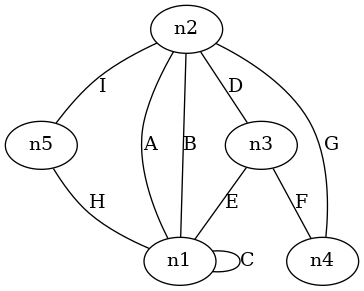
\includegraphics[scale=0.5]{Figures/chapter1/definition_ex_1.png}
\end{center}
  \caption{An undirected pseudograph with labeled nodes and
edges.}\label{fig:SimplePseudograph}

\end{figure}
\begin{example}

  \

For the graph presented in  \fref{fig:SimplePseudograph}  the following
can be assumed:
\begin{align*}
    &G = (V(G), E(G))
    &\intertext{and} 
    &V(G) = \{n_1, n_2, n_3, n_4, n_5\} \\
    &E(G) = \{A, B, C, D, E, F, G, H, I\} 
    &\intertext{and the incidence function is defined as:}
    &\psi_G(A) = n_1n_2,\quad \psi_G(B) = n_1n_2, \quad \psi_G(C) =
      n_1n_1, \quad \psi_G(D) = n_2n_3,\\
    &\psi_G(E) = n_1n_3, \quad \psi_G(F) = n_3n_4, \quad \psi_G(G) = n_2n_4,
      \quad \psi_G(H)= n_1n_5, \\
    &\psi_G(I) = n_2n_5
\end{align*}
\end{example}
  
It should now be clear that with the newer definition of $\phi_G$, self loops are now possible.
Additionaly, even though this was not prohibited by the previous definition, it is worth
noting that a node can be connected to another with multiple edges (or multiedges), or that it can have zero
connections to other nodes. Generally, $V$ is assumed to be a non-empty set, but $E$ can be
empty.

It is now possible to define some characteristic attributes of graphs:
\begin{itemize}
\item $|V|$: the \textbf{order} of a graph is the number of its vertices.
\item $|E|$: the \textbf{size} of a graph is the number of its edges.
\item The \textbf{degree} (or \textbf{valency}) of a single node is the number of
  edges connected to it. The \textbf{degree} of a graph is the maximum number of
  edges connected to a single vertex that belongs to it.
\item The edges of create a \textit{homogenous relation}\footnotemark{} $\sim$ on the vertices
  of the graph that is called \textbf{adjacency relation}; for each edge \textit{$(x, y)$}, its
  endpoints \textit{x, y} are said to be \textbf{adjacent} to each other, denoted by $x \sim y$.
  This property will be particulary useful when the adjacency matrix is defined in the following
  section.
\end{itemize}

\footnotetext{A \textbf{homogenous relation} (or \textbf{endorelation}) over a set \textit{X}
  is a set of assignments (binary relations) over \textit{X} and itself; i.e. it is a subset of
  the cartesian product $X\times X$
}

It can be inferred from the above definitions and attributes that for an undirected
graph of order \textit{n}, the maximum \textit{degree} of a node is $n~-~1$ and
and maximum \textit{size} of a graph is $n(n~-~1)/2$.

\end{definition}

In this section only \textit{undirected} graphs were considered, which are graphs
with edges with no orientation. A whole other class of graph objects with edges which
have orientation exists, called \textit{directed graphs}. These kind of graphs objects
are out of scope for this thesis and will not be presented.


\subsection{Adjacency Matrix}
\begin{definition}
  The \textit{adjacency matrix} is the fundamental mathematical representation of a graph.
  It is a square matrix, the elements of which represent which pair of nodes are
  \textit{adjacent} or not. Thus, the adjacency matrix \textbf{A} of a graph of order $n$
  is the $n\times n$ matrix with elements $A_{ij}$ such that:
  \begin{equation}
    \label{eq:adj_mat}
    A_{ij} = \begin{cases} 1 &\text{if there exists at least one edge connecting $i$ and $j$} \\
               0 &\text{if there no edges connecting those edges directly.}

             \end{cases}
\end{equation}
\end{definition}


\begin{figure}
     \begin{subfigure}[t]{0.4\textwidth}
         \centering
         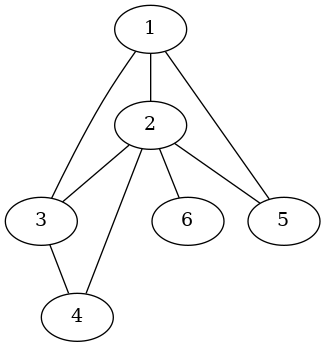
\includegraphics[width=\textwidth]{Figures/chapter1/simple_graph_adj.png}
         \caption{Multigraph with no loops and multiple edges.}
         \label{fig:simple_adj_demo}
     \end{subfigure}
     \hfill
     \begin{subfigure}[t]{0.4\textwidth}
         \centering
         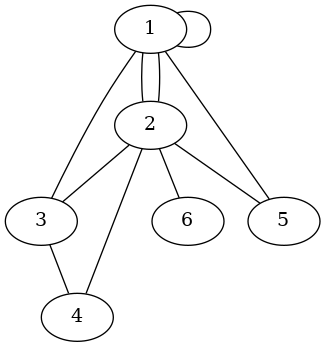
\includegraphics[width=\textwidth]{Figures/chapter1/complex_graph_adj.png}
         \caption{Mutligraph with loops and multiple edges.}
         \label{fig:compl_adj_demo}
     \end{subfigure}
        \caption{Two undirected multigraphs.}
        \label{fig:two multigraphs}
\end{figure}

Considering the simple undirected graph of \fref{fig:simple_adj_demo} we can construct
the following adjacency matrix:
\begin{table}[H]
  
  \begin{equation*}
    A = 
    \begin{pmatrix}
      0 & 1 & 1 & 0 & 1 & 0 \\
      1 & 0 & 1 & 1 & 1 & 1 \\
      1 & 1 & 0 & 1 & 0 & 0 \\
      0 & 1 & 1 & 0 & 0 & 0 \\
      1 & 1 & 0 & 0 & 0 & 0 \\
      0 & 1 & 0 & 0 & 0 & 0 
    \end{pmatrix}
  \end{equation*}
  \caption{Adjacency matrix for \fref{fig:simple_adj_demo}}
\end{table}

For this simple network, which has no loops and only one edge connect two nodes,
the diagonal matrix elements are always zero and the matrix is symmetric, as for
each edge connecting $i$ and $j$ there is a representation for the $j$ to $i$ connection
as well.

In a more complex case, such as the one presented in \fref{fig:compl_adj_demo} where loops
and multiedges are present an adjacency matrix can still be constructed. In this case,
a multiedge is represented by setting the value of the corresponding $A_{ij}$ value equal
to the multiplicity of the edge. In this case, $A_{12} = A_{21} = 2$.

For loops, the most common representation in the case of undirected
graphs is to still set the value of the $A_{ii}$ element equal to $2$
(i.e. $A_{11} = 2$ in the example presented).  Essentially, an edge of
a loop has two ends that connect to the same node, thus the result
\cite[p.~68]{book:algebraic}. Additionaly, defining the matrix in such
manner, allows for better computations and is consistent with the
definition of the representation of an edge connecting two nodes of an
undirected graph \cite[p.~108]{book:Newman}. 

Thus, the adjacency matrix for the graph of \fref{fig:compl_adj_demo} is

\begin{table}[H]
  \begin{equation*}
    A = 
   \begin{pmatrix}
      2 & 2 & 1 & 0 & 1 & 0 \\
      2 & 0 & 1 & 1 & 1 & 1 \\
      1 & 1 & 0 & 1 & 0 & 0 \\
      0 & 1 & 1 & 0 & 0 & 0 \\
      1 & 1 & 0 & 0 & 0 & 0 \\
      0 & 1 & 0 & 0 & 0 & 0 
    \end{pmatrix}
  \end{equation*}
  \caption{Adjacency matrix for  \fref{fig:compl_adj_demo}}
\end{table}
 % Introduction

\chapter{Literature Review} \label{literature}
 % Review of the Literature

\chapter{Notation \& Fundamentals} \label{methodology}
 % Fundamentals

\chapter{Basic Principles and Implementation Framework for an [Problem to be Solved]} \label{framework}
 % Framework

\chapter{Implementation and Core Components of [Platform Title]} \label{platform}
 % Platform

\chapter{Experimentation \& Validation} \label{experimentationANDresults}
 % Experimentation

\chapter{Conclusions \& Future Work} \label{conclusions}
 % Results and Discussion

%\input{Chapters/Chapter7} % Conclusion

%% ----------------------------------------------------------------
% Now begin the Appendices, including them as separate files

\addtocontents{toc}{\vspace{2em}} % Add a gap in the Contents, for aesthetics

\appendix % Cue to tell LaTeX that the following 'chapters' are Appendices

% \chapter{Example Appendix} \label{math}
 
% Example appendices

\addtocontents{toc}{\vspace{2em}}  % Add a gap in the Contents, for aesthetics
\backmatter % End the book's numbering; backpage

%% ----------------------------------------------------------------
\label{Bibliography}
\lhead{\emph{Bibliography}}  % Change the left side page header to "Bibliography"
% \bibliographystyle{ACM-Reference-Format}
\bibliographystyle{unsrtnat}  % Use the "unsrtnat" BibTeX style for formatting the Bibliography
\bibliography{Bibliography}  % The references (bibliography) information are stored in the file named "Bibliography.bib"

\end{document}  % The End
%% ----------------------------------------------------------------
